\begin{figure*}[h]
\begin{center}
  {\small
  \begin{tabular}{cc}
  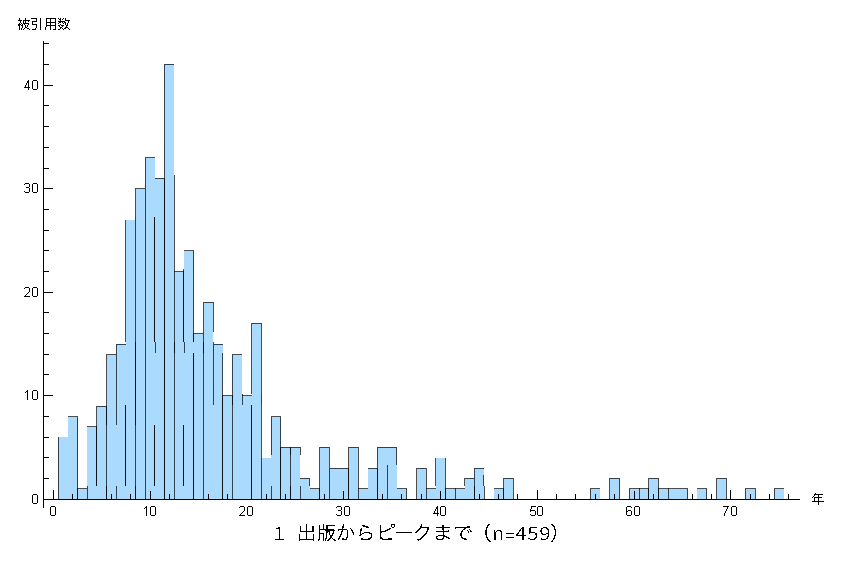
\includegraphics[width=72mm]{obsindex1-1.eps} & 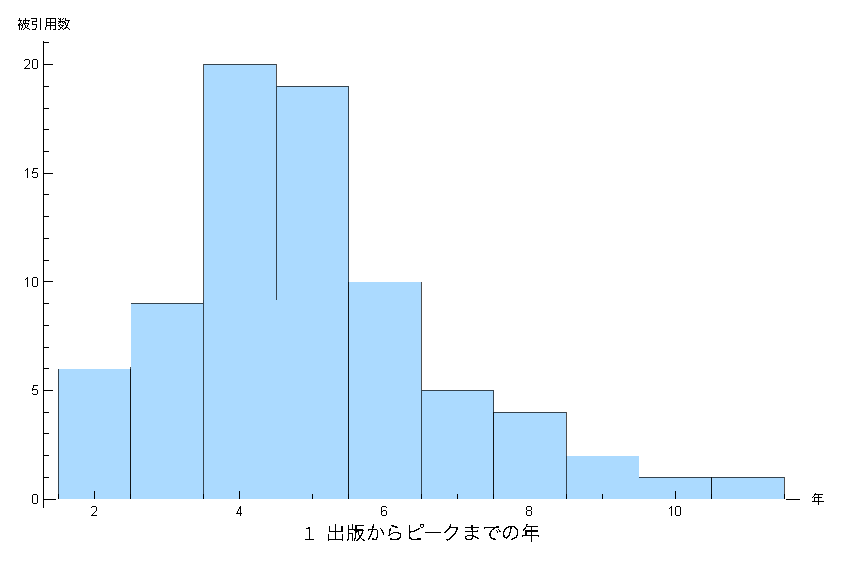
\includegraphics[width=72mm]{obsindex2-1.eps} \\
  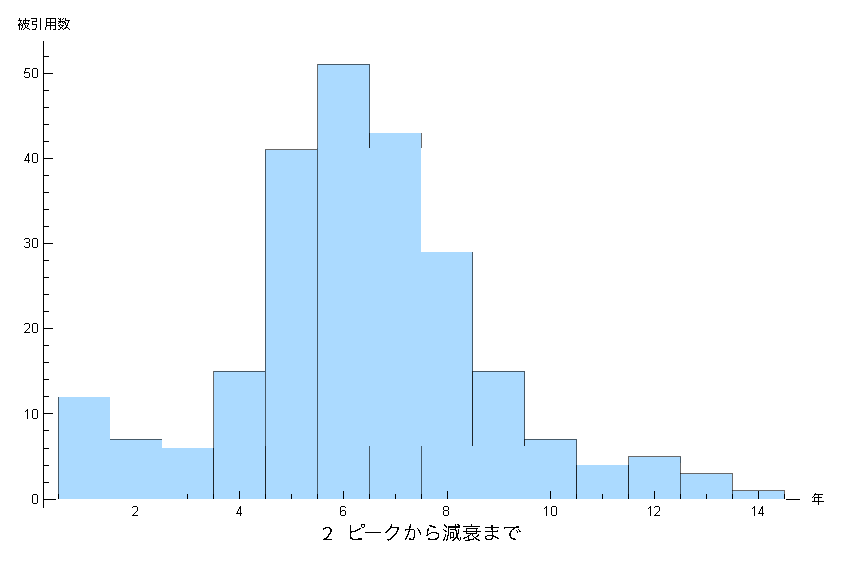
\includegraphics[width=72mm]{obsindex1-2.eps} & 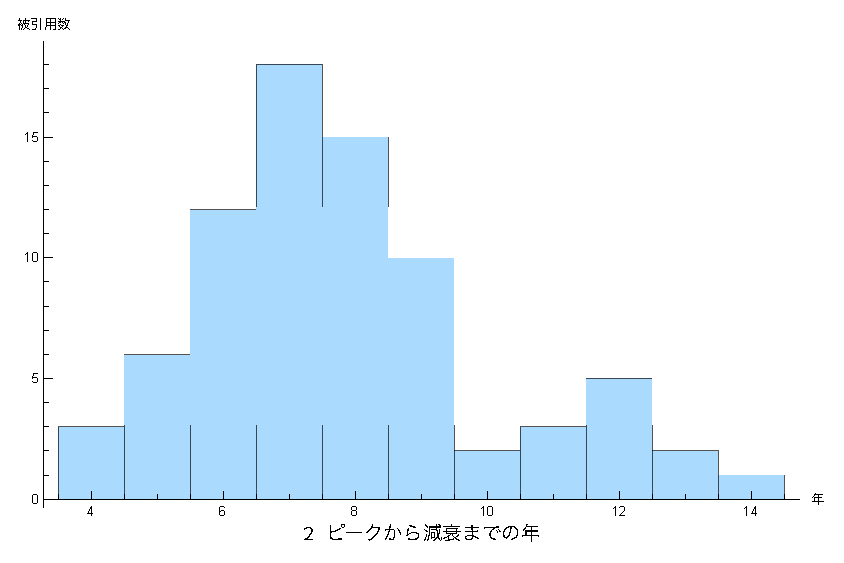
\includegraphics[width=72mm]{obsindex2-2.eps} \\
  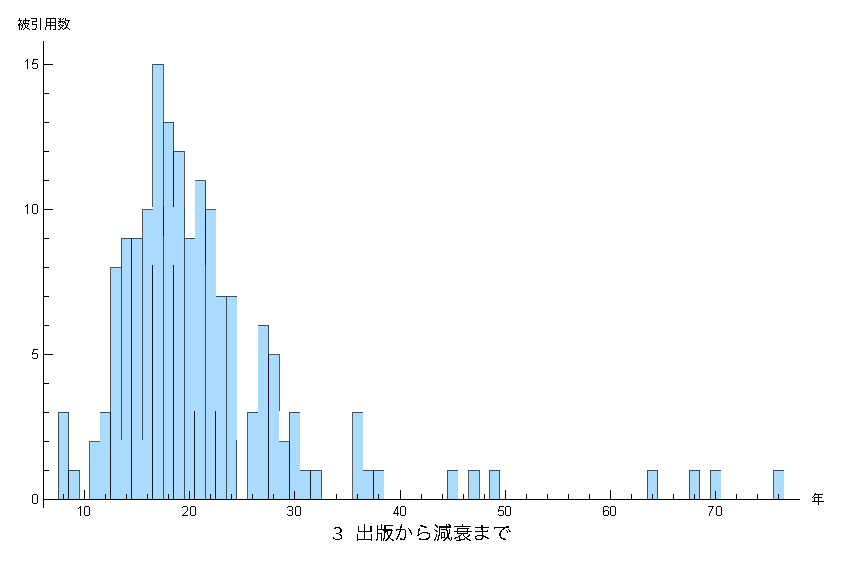
\includegraphics[width=72mm]{obsindex1-3.eps} & 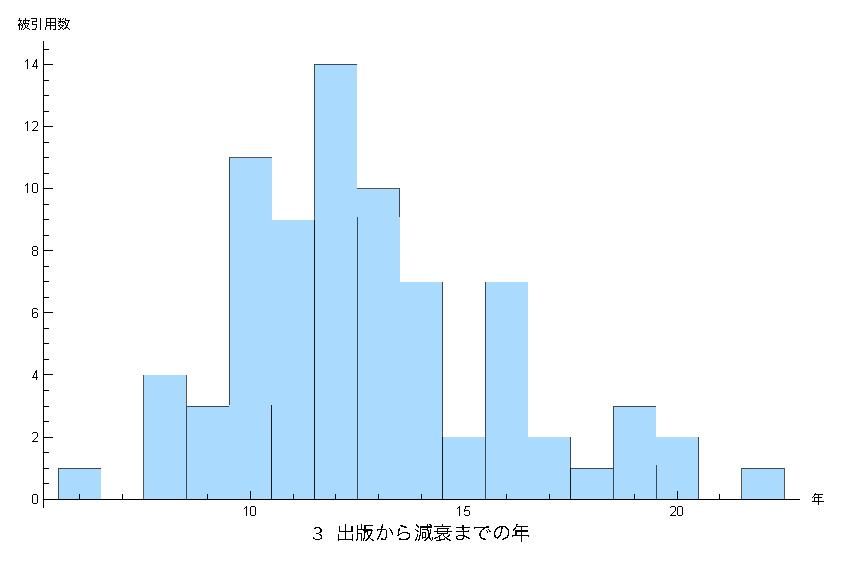
\includegraphics[width=72mm]{obsindex2-3.eps} \\
  {\begin{tabular}{c}1. オブソレッセンス状態にない論文\end{tabular}} & {\begin{tabular}{c}2. オブソレッセンス状態にある論文\end{tabular}} \\
  \end{tabular}
  }
  \caption{高被引用論文のオブソレッセンスにかかる各指標値 \newline 値が算出できない論文は除外している。}
  \label{fig:arr1}
\end{center}
\end{figure*}
